
\documentclass[aps,prl,reprint]{revtex4-2}
\usepackage{gensymb}
\usepackage{wrapfig}
\usepackage{graphicx}
\usepackage{amsmath}
\usepackage{hyperref}
\usepackage{dsfont}
\usepackage{relsize}
\usepackage{wrapfig}
\usepackage{graphicx}
\usepackage{hyperref}
\hypersetup{colorlinks=true, citecolor=blue, urlcolor=blue, linkcolor=blue}


\begin{document}

% Use the \preprint command to place your local institutional report
% number in the upper righthand corner of the title page in preprint mode.
% Multiple \preprint commands are allowed.
% Use the 'preprintnumbers' class option to override journal defaults
% to display numbers if necessary
%\preprint{}

%Title of paper
\title{Hall Effect Lab}

% repeat the \author .. \affiliation  etc. as needed
% \email, \thanks, \homepage, \altaffiliation all apply to the current
% author. Explanatory text should go in the []'s, actual e-mail
% address or url should go in the {}'s for \email and \homepage.
% Please use the appropriate macro foreach each type of information

% \affiliation command applies to all authors since the last
% \affiliation command. The \affiliation command should follow the
% other information
% \affiliation can be followed by \email, \homepage, \thanks as well.
\author{Trevor Smith, Alex Storrer}
\email[]{smith.tr@northeastern.edu}
\homepage[]{https://github.com/trevorm4x/}
%\thanks{}
%\altaffiliation{}
\affiliation{Northeastern University}


\date{\today}

\begin{abstract}
	Nothing is here
\end{abstract}


\maketitle

% body of paper here - Use proper section commands
% References should be done using the \cite, \ref, and \label commands
\section{Introduction}

\section{Apparatus}

The apparatus consisted of the following.

\begin{itemize}
	\item Doped silicon wafer
	\item Pre-wired circuit board
	\item Carbide scribe
	\item 2 soldering iron
	\item Indium solder
	\item Lead-tin solder
	\item Rubber cement
	\item Fine wire
	\item Electromagnet and power supply
	\item Current source (DC power supply)
	\item Two multimeters (for V and I)
\end{itemize}

\section{Make Hall Sample}

\subsection{Procedure}

\begin{wrapfigure}{o}{.28\textwidth}
	\begin{center}
		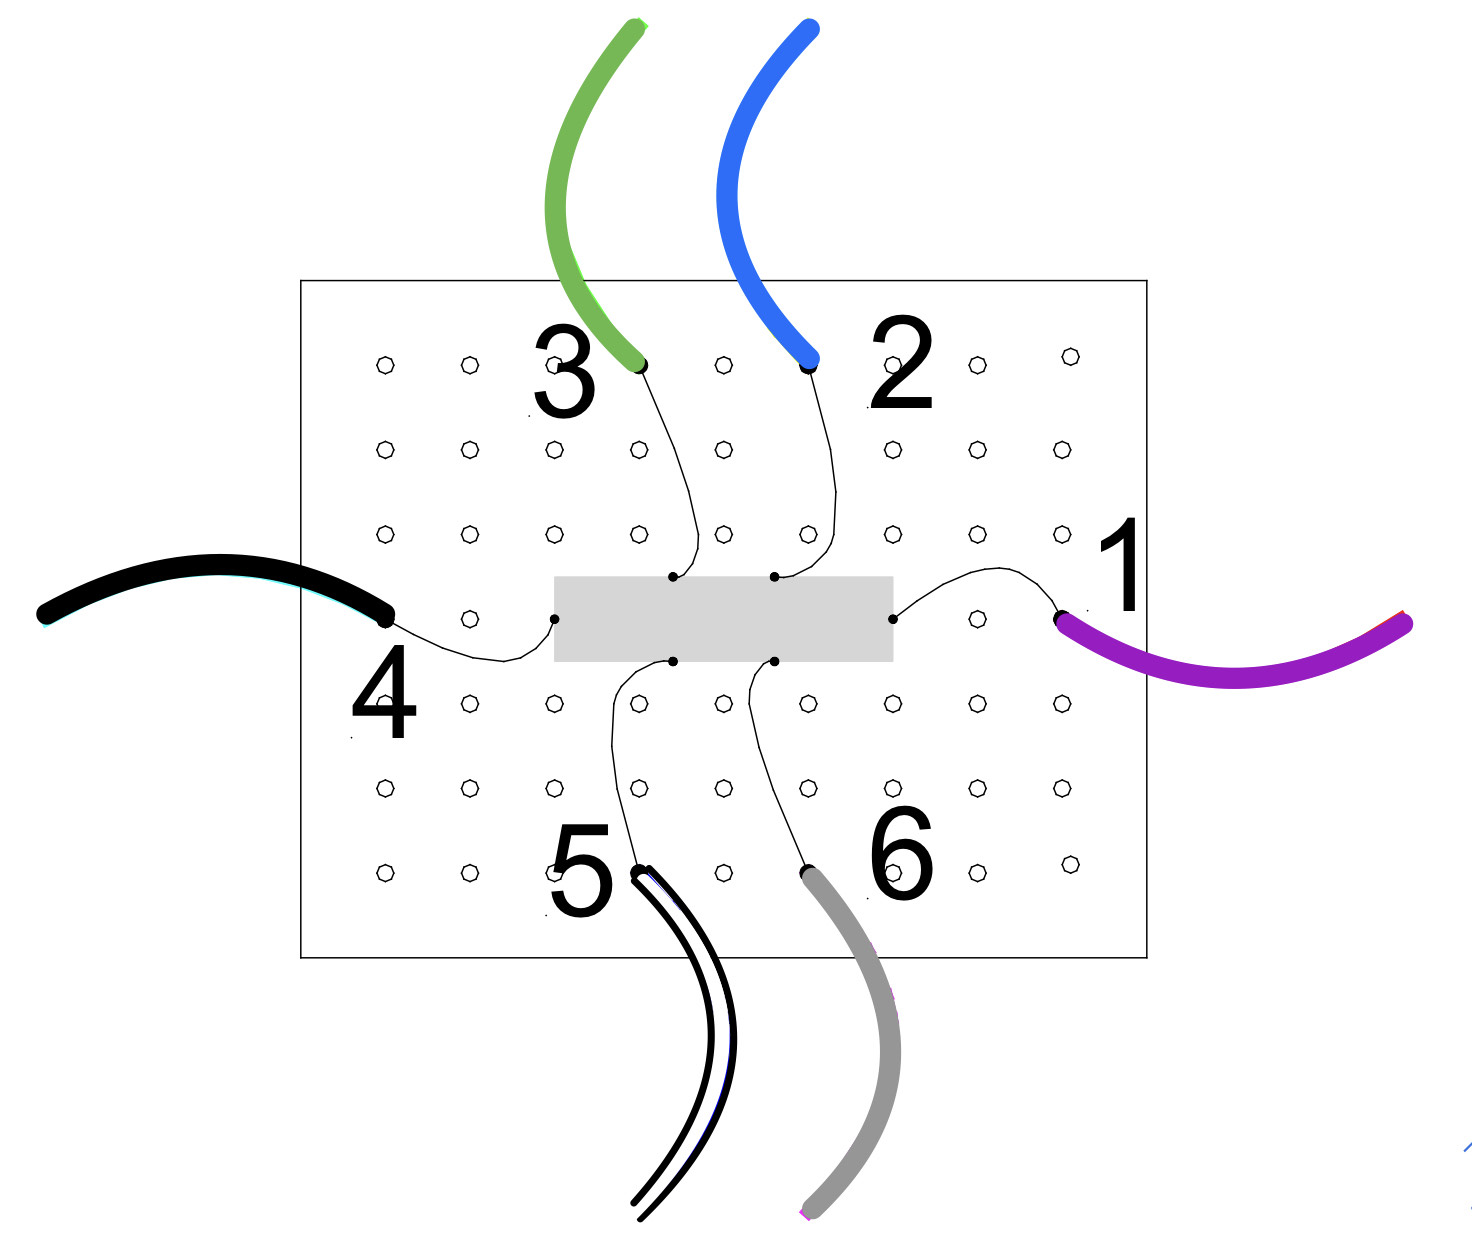
\includegraphics[width=0.29\textwidth]{../Images/l2_WireDiagram.jpg}
	\end{center}
	\caption{\label{colors} Coloring/numbering convention of the experimental setup.}
\end{wrapfigure}

The first step of the experiment was to prepare a hall sample. This involved selecting
and measuring a Si wafer, securing it to a circuit board prefitted with six insulated wires,
and securing the wires to the four sides of the sample with thin wire and indium solder. 
Before soldering, the wafer was measured, width, height, and thickness. 
The configuration of the wires connected to the semiconductor is shown in \ref{colors}. \\

Resistances between each pair of wires was measured with an Ohmeter. One wire was found to have
a bad solder and was resoldered until all measured resistances were $< 1\ M\Omega$. \\

Ohmic behavior was tested by generating a R(V) and I(V) curve. A current was applied to 
the two end wires and varied, such that the resulting power was between -0.1 and 0.1 Watts. \\

\subsection{Results and Conclusion}

Results for the two-wire method of measuring resistance are shown below, where in order to 
measure resistance between two nodes a ohmmeter is simply connected between them. This method
is known to be inaccurate and a more precise method is used later in the experiment, however
this verifies the test setup is correct.

\begin{table}[h]
\begin{tabular}{lr}
\toprule
Wire Pair &  Resistance ($\Omega$) \\
\midrule
\hline
3-2       &     22760.0 \\
3-6       &     24550.0 \\
3-5       &     66430.0 \\
3-4       &     26940.0 \\
3-1       &     28570.0 \\
2-6       &     11213.0 \\
2-5       &     12445.0 \\
2-4       &     12060.0 \\
2-1       &     11665.0 \\
6-5       &     51390.0 \\
6-4       &      8893.6 \\
6-1       &      9566.0 \\
5-4       &    171760.0 \\
5-1       &    176260.0 \\
4-1       &     12296.0 \\
\hline
\hline
\bottomrule
\end{tabular}
\caption{\label{pairs}Resistance for each combination of wires,\\ given by their numbering convention matching that in \ref{colors}.}
\end{table}

Next we probed the behavior of the semiconductor as a resistor, measuring voltage and current as
a voltage was applied, starting at 0 and increasing until the power was just under 0.1 Watts. 

% WHY DOES RESISTANCE

\begin{figure}[h]
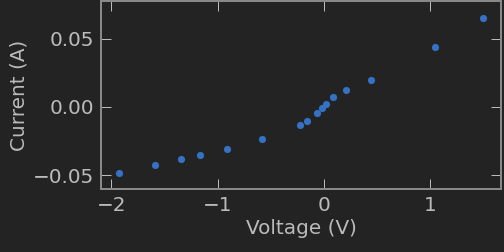
\includegraphics[width=0.5\textwidth]{../Images/l2_a_1.png}
\caption{\label{figA}I(V) shows different behavior closer to zero than elsewhere. }

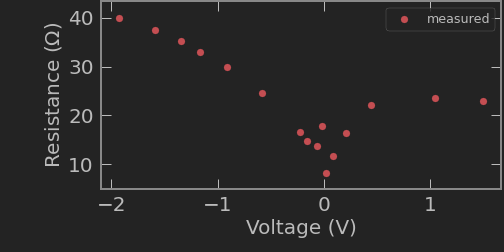
\includegraphics[width=0.5\textwidth]{../Images/l2_a_2.png}
\caption{\label{figA}R(V) is not constant, demonstrating non-ohmic behavior.}
\end{figure}


In this phase of the experiment, we were able to demonstrate that the test setup had no 
major issues and that the behavior of the semiconductor is non-ohmic. This is likely due
to a certain voltage threshold inherent to semiconductors where resistance increases as 
the threshold is approached. If more voltages were able to be tested, we would see a decreasing
trend with increasing voltage after this initial peak.\\

\newpage

\section{The 4-Wire Method for Measuring Resistivity of a Doped Silicon Wafer}

\subsection{Procedure}

\begin{wrapfigure}{o}{.25\textwidth}
	\begin{center}
		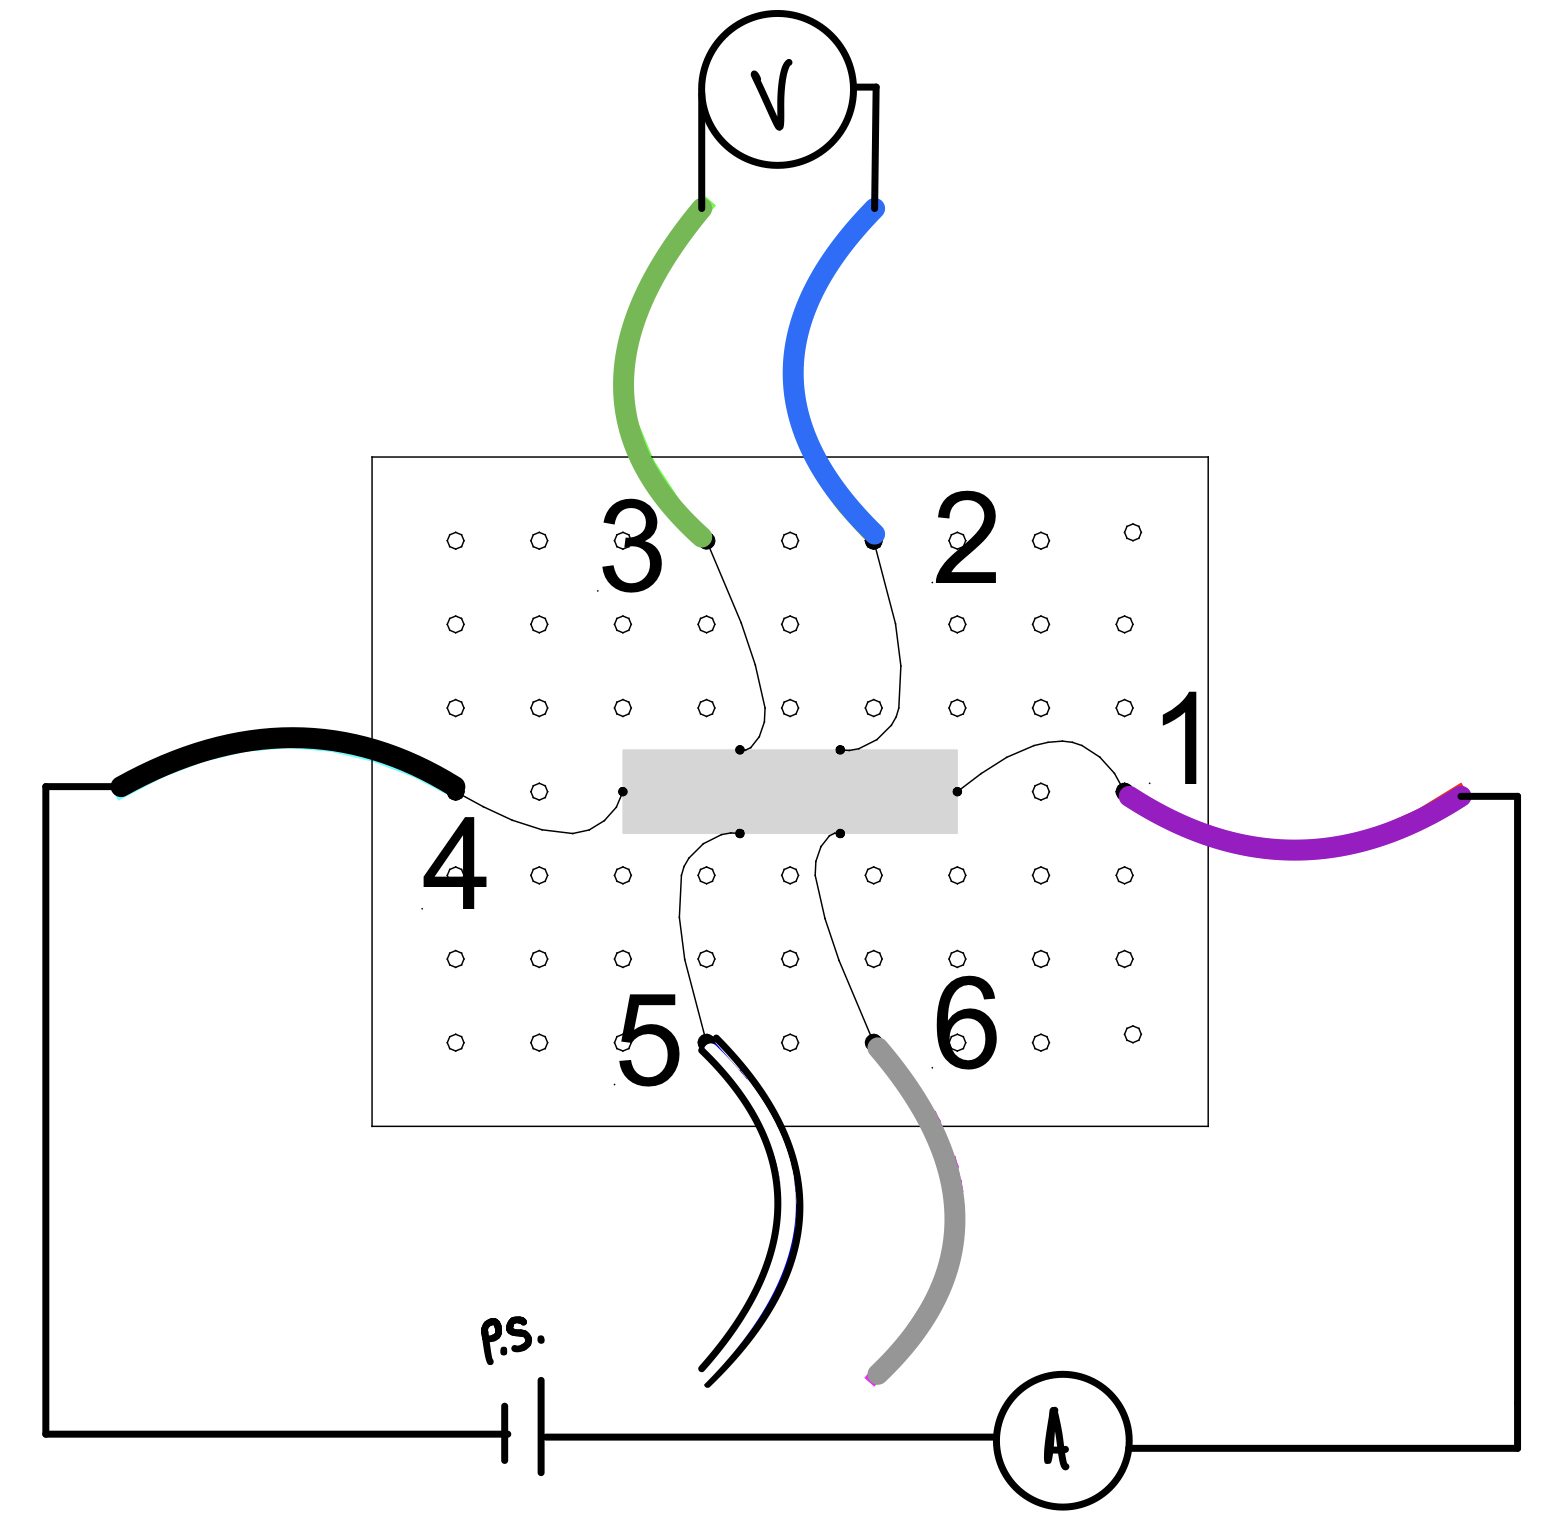
\includegraphics[width=0.29\textwidth]{../Images/l2_4Wire.jpg}
	\end{center}
	\caption{\label{4wire} Four-Wire measurement configuration.}
\end{wrapfigure}

The 4-wire method was used to more accurately measure the resistivity of our material. In this
method, instead of attaching an ohmmeter across the two wires, resulting in a resistivity
that includes the wires and connections between said wires, two measurements that are 
orthagonal are performed. An ampmeter is used to measure an applied current across the same
two wires (which gives an accurate measure of current because the circuit is isolated along 
that path), and a voltmeter is used to measure immediately along either side of the resistor,
in this case across wires 2-3 and 5-6, where any resistance does not cause a meaningful 
voltage drop.\\

These values for resistance were then used to calculate the material's resistivity $\rho$,
using the earlier measurements of the wafer's dimensions. \\

Finally, measurements across the side wires were repeated with the ohmmeter for comparison. \\

\subsection{Results and Conclusion}

Two values for $\rho$ were attained using equation \ref{rho}, and a comparison was
made between the two methods for measuring resistance, given in table \ref{rhotable}. 

\begin{equation}
	\mathlarger{\rho=\frac{R\cdot A}{L}}
    \label{rho}
\end{equation}

\begin{table}[h!]
\renewcommand{\arraystretch}{1.45}
\setlength{\tabcolsep}{10pt}
\begin{tabular}{lrrr}
\toprule
Path &  4-Wire R ($\Omega$) &  2-Wire R ($\Omega$) &       $\rho\ (m\Omega)$ \\
\midrule
2-3 &         147 &     20200.0 &  0.079131 \\
5-6 &         235 &    213600.0 &  0.102832 \\
\bottomrule
\end{tabular}
\end{table}
There is indeed a substantial difference between the two measuring methods in this case,
three orders of magnitude. Additionally, the two 4-wire measurements were different by about 2x,
but the 2-wire measurements were different by an order of magnitude. Thus, the relative variance
of the 2-wire method is much higher, implying that it has both worse accuracy and precision.\\

This is of course due mostly to the quality of the solder connections between the wires and the
semiconductor, meaning that the connections on one side were probably just worse than the other 
side.\\

Because two measurements of $\rho$ were calculated, which are both measuring the same property
of the same material, they were taken as a small distribution, with the mean as the measured
value and the uncertainty the standard deviation. Our measured value is therefore
$9\ \pm\ 2\ cm\Omega$.

\section{Summary}

\begin{widetext}
\begin{center}
\begin{table}[h]
\renewcommand{\arraystretch}{1.35}
\setlength{\tabcolsep}{10pt}
\caption{\label{rhotable}Measured and accepted values of the speed of light and refractive index of various materials.}
\begin{tabular}{ccccc}
%\hline
\toprule
Property & Measured Value &  Accepted Value & Refs. &   Deviation \\
\colrule
$\rho$ &    $0.09 \pm 0.02\  (cm\Omega)$ &  $5.86-6.31\ (cm\Omega)$ &  \cite{resistivity} &   $2\sigma$ \\
\colrule
$\mu$ &  $320 \pm 60\  (\frac{cm}{Vs})$ &      $455\ (\frac{cm}{Vs})$ &  \cite{resistivity} &  $-3\sigma$ \\
%\hline
\botrule
\end{tabular}
\end{table}
\end{center}
\end{widetext}


\begin{thebibliography}{9}
%
\bibitem{HHV} 
Wikipedia, Heat of Combustion: \\
\href{https://en.wikipedia.org/wiki/Heat_of_combustion}{https://www.wikepedia.com}
%
\bibitem{Solar Cell} 
Energysage, Most Efficient Solar Panels\\
\href{https://news.energysage.com/what-are-the-most-efficient-solar-panels-on-the-market/#:~:text=How%20efficient%20are%20solar%20panels,are%20not%20above%2020%25%20efficiency.}{https://www.energysage.com/}
%
\bibitem{Electrolyzer} 
Carbon Commentary, Hydrogen made by Electolysis\\
\href{https://www.carboncommentary.com/blog/2017/7/5/hydrogen-made-by-the-electrolysis-of-water-is-now-cost-competitive-and-gives-us-another-building-block-for-the-low-carbon-economy}{https://www.carboncommentary.com}
%

%
\bibitem{Fuel Cell} 
Energy.gov, Fuel Cell Fact Sheet\\
\href{https://www.energy.gov/sites/prod/files/2015/11/f27/fcto_fuel_cells_fact_sheet.pdf}{https://www.energy.gov}

\end{thebibliography}


\end{document}
%
% ****** End of file apstemplate.tex ******

